% !TEX root = rob1.tex
\chapter{Umweltmodellierung}

\section{Objektmodelle}
\subsection{Kantenmodelle}
\begin{compactitem}
    \item Nur die Kanten werden gespeichert, d.h. Punkte und Verbindungen (Geraden, Polygonzug, Bezierkurve)
    \item \textbf{Vorteile}:
    \begin{compactitem}
        \item einfache Daten
        \item wenige Daten
    \end{compactitem}
    \item \textbf{Nachteile}:
    \begin{compactitem}
        \item Mehrdeutigkeiten
        \item hoher Eingabeaufwand
        \item keine Kollisionsberechnung
        \item kein Schnitt
    \end{compactitem}
\end{compactitem}
\subsection{Flächenmodelle}
\begin{compactitem}
    \item Speicherung von Kanten und Oberflächen (Dreiecke, Bezier)
    \item \textbf{Vorteile}:
    \begin{compactitem}
        \item effiziente Verfahren
        \item entspricht dem Vorgehen während der Modellierung
        \item schnelle Kollisions und Abstandsberechnung
    \end{compactitem}
    \item \textbf{Nachteile}:
    \begin{compactitem}
        \item hoher Eingabeaufwand
        \item Darstellung aufwendig
        \item Problem bei Schnittoperationen
        \item Inkonsitenz möglich
    \end{compactitem}
\end{compactitem}

\mparagraph{Boundary Representation}
Hierarchische Darstellung eines Objektes durch begerenzte Elemente i.d.R Kanten oder Flächen. \\
Beispiel: Elemente eines Quaders im Flächenmodell
\begin{compactitem}
    \item $Q$: Quader
    \item $F_i : i \in \{1,...,6\}$: Flächen
    \item $K_i : i \in \{1,...,12\}$: Kanten
    \item $P_i : i \in \{1,...,8\}$: Ecken
\end{compactitem}
Darstellung in einer topologischen Struktur. Liefert Information über:
\begin{compactitem}
    \item Welche Flächen gehören zum Objekt
    \item Welche Kanten gehören zur Fläche
    \item Zu welchem Objekt gehört eine Kante
    \item Zu welchem Objekt gehört eine Fläche
    \item Welche Flächen stoßen aneinandern?
\end{compactitem}
\subsection{Volumenmodelle}
\subsubsection{A. Punktwolken}
\begin{compactitem}
    \item einfachstes Objektmodell
    \item Modell ist eine beliebige Menge aus Raumpunkten
    \item Daten direkt aus aktuellen Tiefensensoren
    \item Objekt nur implizit, indirekt modelliert
    \item Mehrdeutigkeit
\end{compactitem}
\subsubsection{B. Approximative Oberflächen}
\begin{compactitem}
    \item Bildung einer großen Fläche aus einem Netz von einfachen Einzelflächen
    z.B Dreiecke, Vierecke
    \item \textbf{Vorteile}
    \begin{compactitem}
        \item Definition sehr einfach
        \item einfache Algorithmen
    \end{compactitem}
    \item \textbf{Nachteile}
    \begin{compactitem}
        \item hoher Speicherbedarf
        \item hoher Rechenaufwand
    \end{compactitem}
\end{compactitem}
\mparagraph{Dreiecksfläche}
Approximation von Freiformflächen. Gegeben sind 3 Punkte im Raum $P_1, P_2, P_3$. Dann gilt für die
Fläche: $F(u,v) = u \cdot P_1 + v \cdot P_2 + (1-u-v) \cdot P_3$ mit $0 \leq u,v,u+v \leq 1$
\mparagraph{Bilineare Vierecksflächen}
Fläche ist wie folgt definiert bei 4 gegebenen Punkten im Raum: $F(u,v) = (1-u)(1-v) \cdot P_1 +
(1-u)v \cdot P_2 + u(1-v) \cdot P_3 + uv \cdot P_4$ mit $0 \leq u \leq 1, 0 \leq v \leq 1$
\begin{compactitem}
    \item \textbf{Vorteile}: Flächen können gekrümmt sein. Somit weniger Gitterpunkte bei gleich guter
    Approximation
    \item \textbf{Nachteile}: Rechnen mit gekrümmten Flächen ist aufwendig
\end{compactitem}

\mparagraph{Bezierflächen}
Erweiterung des Ansatzes der Bezierkurven. Gegeben ist ein Gitter mit Führungspunkten $P_{ij},
0 \leq i \leq N$ und $0 \leq j \leq M$
\begin{align}
    F(u,v) &= \sum_{i=0}^N\sum_{j=0}^M  P_{ij} \cdot B_{i,N}(u) \cdot B_{j,M}(v) \\
    B_{i,N}(u) &= (1-u)B_{i,N-1}(u) + u \cdot B_{i-1,N-1}(u)  \\
    B_{j,M}(v) &= (1-v)B_{j,M-1}(v) + v \cdot B_{j-1,M-1}(v)
\end{align}
\subsubsection{Approximative Zellenbelegung}
\mparagraph{A. Voxel}
Objekte werden aus disjunkten Elementarzellen aufgebaut. (Tetraeder, Quader)
\begin{compactitem}
    \item \textbf{Vorteile}:
    \begin{compactitem}
        \item Einfache Darstellung
        \item Berechnung homogen, parallel auf GPU
        \item Raycasting u.ä einfach parallelisierbar
    \end{compactitem}
    \item \textbf{Nachteile}:
    \begin{compactitem}
        \item Festes Gitter, gleicher Detaillierungsgrad sowohl bei großflächigen als auch feiner
        aufgelösten Strukturen
        \item Kartengröße/Präzision durch Speicher begrenzt
    \end{compactitem}
\end{compactitem}
\mparagraph{B. Octree}
\begin{compactitem}
    \item Raum wird in mehrere Zellen unterteilt
    \item Zelle komplett vom Objekt belegt $\rightarrow$ als belegt markieren
    \item Zelle teilweise belegt, dann weiter unterteilen und wiederholen, sonst leer
    \item Rekursion terminiert bei einer vorbestimmten minimalen Zellgröße
    \item Teilbelegt kleinste Zellen werden als belegt markiert
\end{compactitem}
\subsubsection{Analytisch Paramterische Modelle}
Grundkörper und topologische Operationen auf diesen werden abgespeichert. \\
\begin{compactitem}
    \item \textbf{Vorteile}:
    \begin{compactitem}
        \item Eindeutige Objektbeschreibung
        \item Geringer Eingabeaufwand
        \item Ergebnis vo Operationen sind korrekte Objekte
    \end{compactitem}
    \item \textbf{Nachteile}:
    \begin{compactitem}
        \item hoher Implementierungsaufwand
        \item Einbindung von Freiformflächen schwierig
    \end{compactitem}
\end{compactitem}
\mparagraph{Constructive Solid Geometry, CSG}
Objekte sind bereits vorhanden und können durch Angabe von Parametern angepasst werden (Varianten) z.B
\begin{compactitem}
    \item \textbf{Körper}
    \begin{compactitem}
        \item \textbf{Quader}: Länge, Breite, Höhe
        \item \textbf{Prisma}: Länge, Radius, Facettem
        \item \textbf{Zylinder}: Länge Radius
        \item \textbf{Kegel}: Länge, Radius a, Radius b
        \item \textbf{Ellipsoid}: Radius a, Radius b, Radius c
    \end{compactitem}
    \item \textbf{Operatoren}
    \begin{compactitem}

        \item \textbf{Vereinigung}: $A \cup B$
        \item \textbf{Schnitt}: $A \cap B$
        \item \textbf{Differenz}: $A / B$
        \item \textbf{Sweep}: Ein Grundelement wird entlang einer Raumkurve geschoben. Der durchdrungene
        Raum stellt das neue Objekt dar.
        \item Speicherung erfolgt als Binärbaum mit Knoten als Operation und Teilbaum als Teil-CSG oder
        Grundkörper
    \end{compactitem}
\end{compactitem}

\section{Umwandlung}
\begin{figure}[!h]
    \centering
    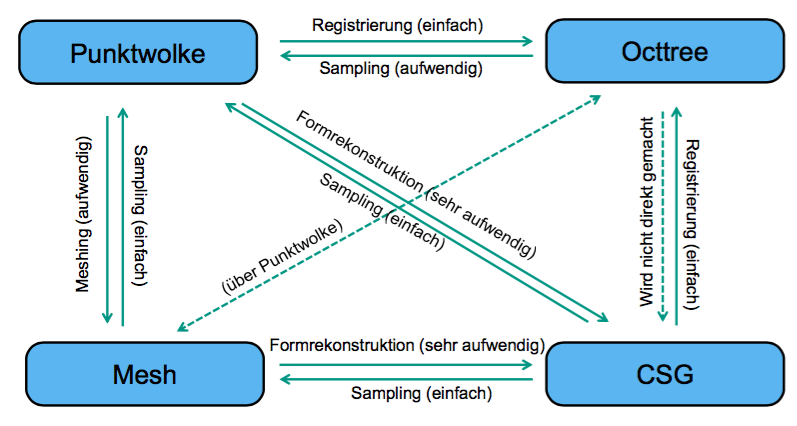
\includegraphics [scale=0.5]{umwandlung}
\end{figure}
